\chapter{[必须安装Excel] xlwings库}

\section{简介}
使用xlwings\textcolor{red}{\textbf{必须}}安装Excel软件，xlwings是一个用于在Excel中调用Python的库，

\subsection{xlwings的数据结构}
\begin{figure}[htpb]
    \centering
    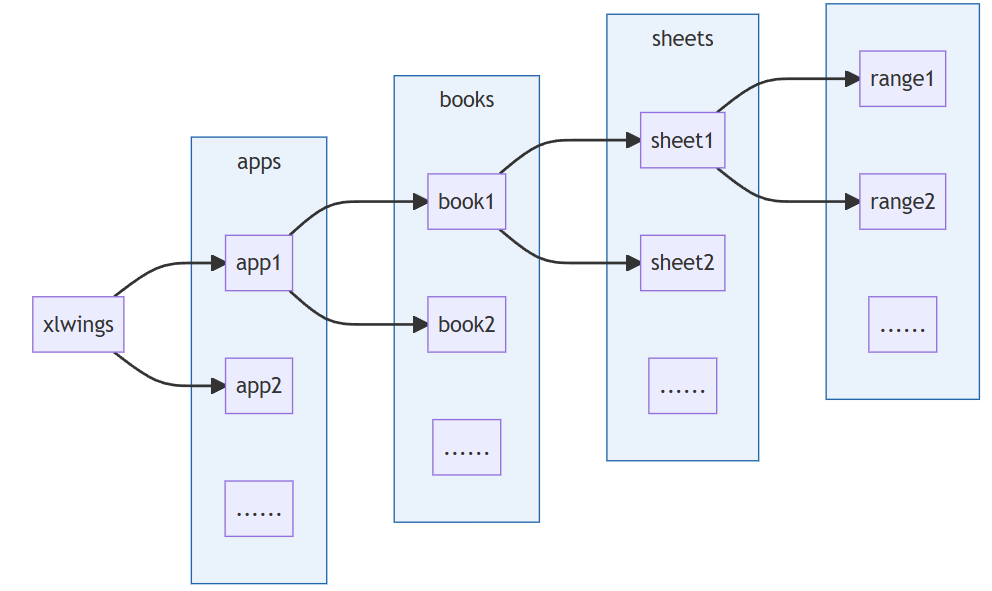
\includegraphics[width=0.6\textwidth]{part/自动化/办公自动化/pic/excel/xlwings/xlwings的数据结构.png}
    \caption{xlwings的数据结构}
    \label{fig:xlwings的数据结构}
\end{figure}
如图\ref{fig:xlwings的数据结构}所示，xlwings的数据结构主要有以下几个部分：
\begin{enumerate}[label=\arabic*)]
    \item App：单个Excel程序
    APP可以是一个Excel的实例，在此实例下创建工作薄，要创建工作簿，就必须先创建App实例。

    APP也可以是Excel程序集合,
    使用xlwings可以创建一个或者多个App,多个App之间是相互独立的,每个App对应一个PID值，PID值是数字编号，可以用来识别不同的App
    
    \item Book：单个工作簿

    \item Sheet：工作表

    \item Range: 单元格范围

\end{enumerate}


\section{安装}
\begin{lstlisting}[style=demostyle,numbers=none]
# pip 安装
pip install xlwings

pip install xlwings -i https://pypi.tuna.tsinghua.edu.cn/simple
# conda 安装
conda install xlwings
\end{lstlisting}

\section{App应用程序}
也正是因为App的存在，所以\codeinline{xlwings}必须安装Excel软件，否则无法使用xlwings库。

\begin{lstlisting}[style=demostyle,numbers=none]
import xlwings as xw
## App打开Excel
## visible = True 显示Excel界面
## add_book = False 不添加新的工作簿
app = xw.App(visible = True, add_book = False) 
# app = xw.App(visible = False, add_book = False) 

app.quit() # 关闭Excel
\end{lstlisting}

虽然新版的xlwings,可以直接对Book进行操作，
但是功能很有限，所以还是建议使用App来操作Excel。

\section{Book工作簿(Excel文件)}
工作簿的含义是Excel文件，可以通过xlwings创建一个新的工作簿

\subsection{新建/保存关闭工作簿}
\begin{lstlisting}[style=demostyle,numbers=none]
import xlwings as xw

# 1.创建一个新的工作簿
app = xw.App(visible = True, add_book = False) 
## 1.2 创建一个新的工作簿
wb = app.books.add()

# 2.保存工作簿
wb.save('test.xlsx')
wb.close() # 关闭工作簿
app.quit() # 关闭Excel
\end{lstlisting}

\subsection{获取当前活动工作簿}
\begin{lstlisting}[style=demostyle,numbers=none]
import xlwings as xw

# 获取当前活动的工作簿
active_wb = xw.books.active
\end{lstlisting}


\begin{lstlisting}[style=pythonstyle,numbers=left]
import xlwings as xw

app = xw.App(visible=True, add_book=False)
for i in range(1, 21):
    # 新建工作簿
    workbook = app.books.add()

    # 保存为特定文件名
    file_path = f'c:\\Users\\bingx\\Documents\\Python\\分公司{i}.xlsx'
    workbook.save(file_path)


    # 输出保存的文件路径（或名称）
    # print(f"已保存: {file_path}")
    
    workbook = app.books.open(file_path)  # 重新打开
    print(f"当前工作簿: {workbook.name}")

    # 关闭工作簿
    workbook.close()

# 关闭 Excel 应用
app.quit()
\end{lstlisting}
\begin{lstlisting}[style=demostyle,numbers=none]
前工作簿: 分公司1.xlsx
当前工作簿: 分公司2.xlsx
当前工作簿: 分公司3.xlsx
当前工作簿: 分公司4.xlsx
当前工作簿: 分公司5.xlsx
当前工作簿: 分公司6.xlsx
当前工作簿: 分公司7.xlsx
当前工作簿: 分公司8.xlsx
当前工作簿: 分公司9.xlsx
当前工作簿: 分公司10.xlsx
当前工作簿: 分公司11.xlsx
当前工作簿: 分公司12.xlsx
当前工作簿: 分公司13.xlsx
当前工作簿: 分公司14.xlsx
当前工作簿: 分公司15.xlsx
当前工作簿: 分公司16.xlsx
当前工作簿: 分公司17.xlsx
当前工作簿: 分公司18.xlsx
当前工作簿: 分公司19.xlsx
当前工作簿: 分公司20.xlsx
\end{lstlisting}

\subsection{删除工作簿}
xlwings 本身不能直接删除文件，但你可以结合 Python 的 \codeinline{os} 模块实现：
\begin{lstlisting}[style=demostyle,numbers=none]
import os

# 删除文件
file_path = 'test.xlsx'
os.remove(file_path)
\end{lstlisting}


\section{Sheet工作表(sheet)}
\subsection{新建工作表(sheet)}
\begin{lstlisting}[style=demostyle,numbers=none]
import xlwings as xw

# 1.创建一个新的工作簿
app = xw.App(visible = True, add_book = False) 
wb = app.books.add()

# 2.新建一个工作表
## 2.1 根据索引新建工作表
worksheet = wb.sheets[0] # 获取第一个工作表
worksheet.name = '员工信息' # 设置工作表的名称
## 2.2 在开头插入新的工作表
worksheet = wb.sheets.add('产品统计表') # 添加一个新的工作表
# 2.3在指定位置插入新的工作表
worksheet = wb.sheets.add('产品销售表', after='员工信息') # 添加一个新的工作表

# 3.保存工作簿
wb.save('test.xlsx')
wb.close() # 关闭工作簿
app.quit() # 关闭Excel
\end{lstlisting}
\begin{figure}[htpb]
    \centering
    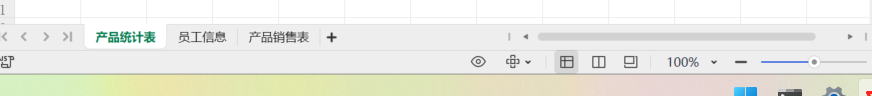
\includegraphics[width=0.4\textwidth]{part/自动化/办公自动化/pic/excel/xlwings/新建工作表演示.png}
    \caption{新建工作表演示}
    \label{fig:新建工作表演示}
\end{figure}

\subsubsection{获取工作表(sheet)}
\begin{enumerate}[label=\arabic*)]
    \item 按索引：\codeinline{wb.sheets[索引值]}, \textcolor{YBXPurple}{索引值从0开始}
    \item 按名称：\codeinline{wb.sheets['工作表名']}
    \item 当前活动工作表：\codeinline{wb.sheets.active}
    \item 获取所有工作表：\codeinline{wb.sheets}（返回所有工作表的集合）
\end{enumerate}

\subsubsection{按索引/名称获取工作表}
\begin{lstlisting}[style=demostyle,numbers=none]
import xlwings as xw

# 打开工作簿
wb = xw.Book('example.xlsx')

# 1.获取第一个工作表（索引从 0 开始）
sheet = wb.sheets[0]
print(sheet.name)  # 打印工作表名称

# 2.获取名为 'Sheet1' 的工作表
sheet = wb.sheets['Sheet1']
print(sheet.name)

# 3.获取当前活动的工作表
active_sheet = wb.sheets.active
print(active_sheet.name)
\end{lstlisting}


\subsection{获取工作簿中所有工作表}
\begin{lstlisting}[style=demostyle,numbers=none]
import xlwings as xw
wb = xw.Book("xlsx路径")
sheets = wb.sheets
\end{lstlisting}

\begin{lstlisting}[style=pythonstyle,numbers=left]    
import xlwings as xw
# 
wb = xw.Book("openpyxl/吉林2024-2021招生录取2024.11.14日姚老师校对基础表.xlsx")

# 获取工作簿中的所有工作表
sheets = wb.sheets

# 打印所有工作表的名称
print("工作簿中的所有工作表:")
for sheet in sheets:
    print(sheet.name)

# 关闭工作簿
wb.close()
\end{lstlisting}
\begin{lstlisting}[style=demostyle,numbers=none]
工作簿中的所有工作表:
录取表
普通专科物理
普通专科历史
普通本科物理
普通本科历史
提前A物理
提前A历史
查找表
错误名称表
\end{lstlisting}
\begin{figure}[htpb]
    \centering
    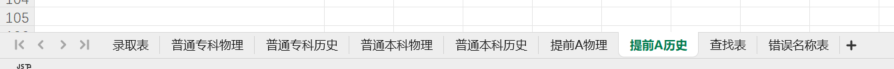
\includegraphics[width=0.6\textwidth]{part/自动化/办公自动化/pic/excel/xlwings/获取工作簿中所有工作表.png}
    \caption{获取工作簿中所有工作表}
    \label{fig:获取工作簿中所有工作表}
\end{figure}

\subsection{删除工作表(sheet)}
\begin{enumerate}[label=\arabic*)]
    \item 先获取工作表对象
    \item 然后调用 \codeinline{.delete()} 方法
\end{enumerate}

\begin{lstlisting}[style=demostyle,numbers=none]
# 删除指定工作表
sheet_to_delete = wb.sheets['Sheet1']
sheet_to_delete.delete()        
\end{lstlisting}

\subsection{重命名工作表}
\begin{enumerate}[label=\arabic*)]
    \item 先获取工作表对象
    \item 然后调用 \codeinline{.name} 属性
\end{enumerate}
\begin{lstlisting}[style=demostyle,numbers=none]
# 重命名工作表
sheet_to_rename = wb.sheets['Sheet1']
sheet_to_rename.name = '新名词'        
\end{lstlisting}

\section{Range区域/单元格}
具体对某个 Sheet 中行、列、单元格的操作，都是通过 \codeinline{sheet} 对象来实现的。
\subsection{获取单元格}
使用\codeinline{sheet.range}方法获取单元格，\codeinline{range}方法的参数可以是单元格的坐标，也可以是单元格的范围。
\begin{lstlisting}[style=demostyle,numbers=none]
# 获取单个单元格
cell = sheet.range('A1')

# 获取多个单元格
cells = sheet.range('A1:B3')
\end{lstlisting}

\begin{enumerate}[label=\arabic*)]
    \item 如果是单个单元格，返回的是 \codeinline{Range} 对象
    \item 如果多个单元格是一行/列，返回的是该行/列的 \codeinline{Range} 对象
    \item 如果多个单元格是一个矩形区域，返回的是该矩形区域的 \codeinline{Range} 对象，如图\ref{fig:xlwings_range获取某一区间}所示
\end{enumerate}

如果要获取单元格的值，可以使用 \codeinline{range.value} 属性：

\begin{figure}[htpb]
    \centering
    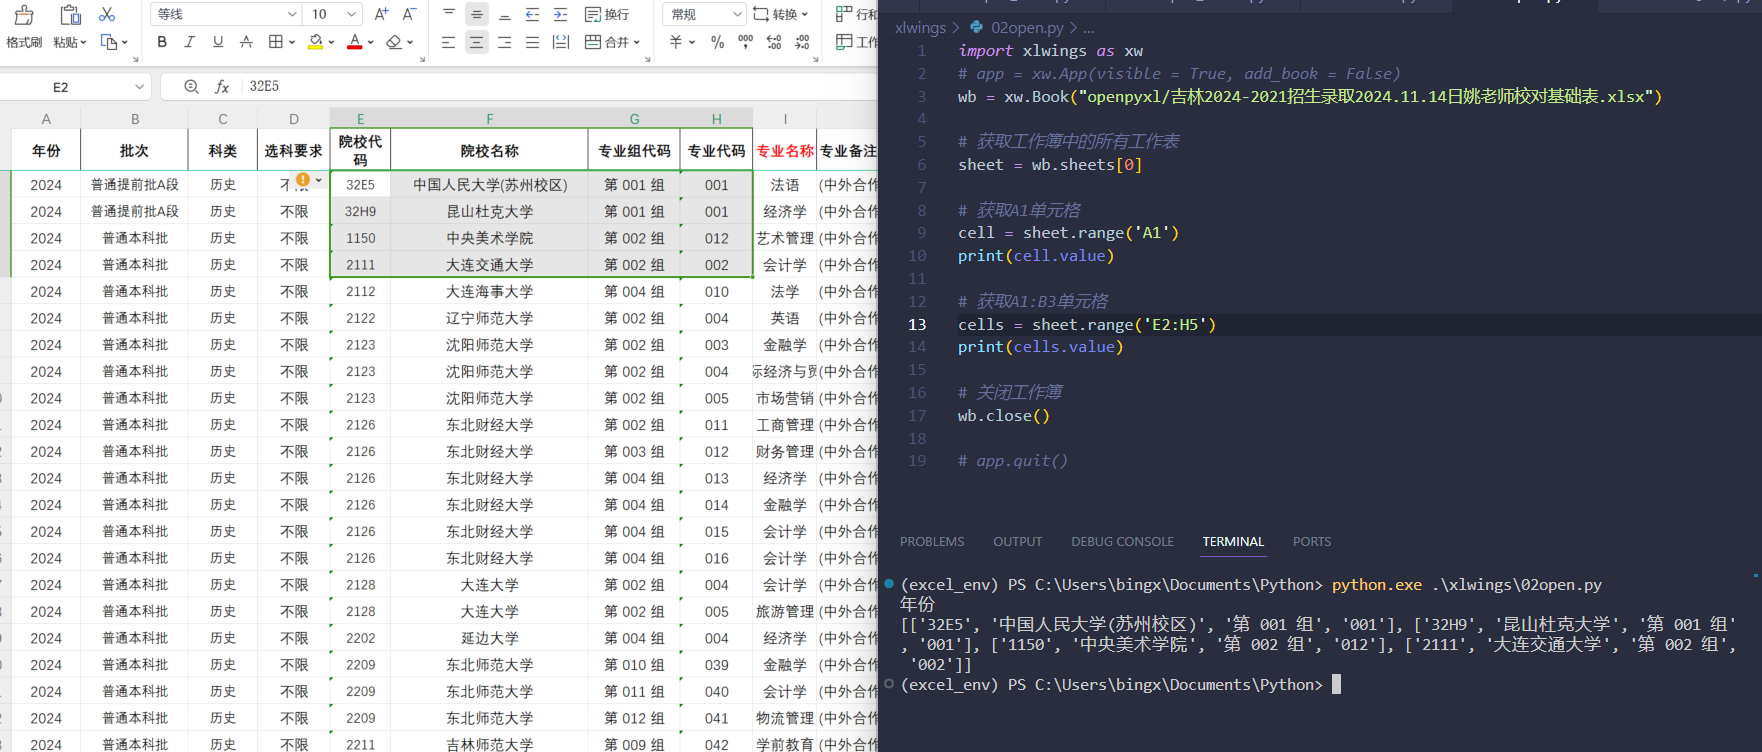
\includegraphics[width=0.6\textwidth]{part/自动化/办公自动化/pic/excel/xlwings/range获取某一区间.png}
    \caption{range获取某一区间}
    \label{fig:xlwings_range获取某一区间}
\end{figure}

\begin{lstlisting}[style=demostyle,numbers=none]
# 读取整行
row_values = sheet.range('1:1').value

# 读取整列
col_values = sheet.range('A:A').value
\end{lstlisting}

\subsection{清除单元格}
清除单元格的方法是 \codeinline{range.clear\_contents()},仅清除单元格内容（文字、数字、公式等）。
不改变工作表的结构（例如行列位置保持不变）。
\begin{lstlisting}[style=pythonstyle,numbers=left]   
import xlwings as xw

app = xw.App(visible=False, add_book=False)
wb = xw.Book("openpyxl/吉林2024-2021招生录取2024.11.14日姚老师校对基础表.xlsx")
sheet = wb.sheets[0]

# 清空A1:C3范围内的单元格
sheet.range('A1:C3').clear_contents()

wb.save("openpyxl/clear_contents.xlsx")
wb.close()
app.quit()
\end{lstlisting}

\begin{figure}[htpb]
    \centering
    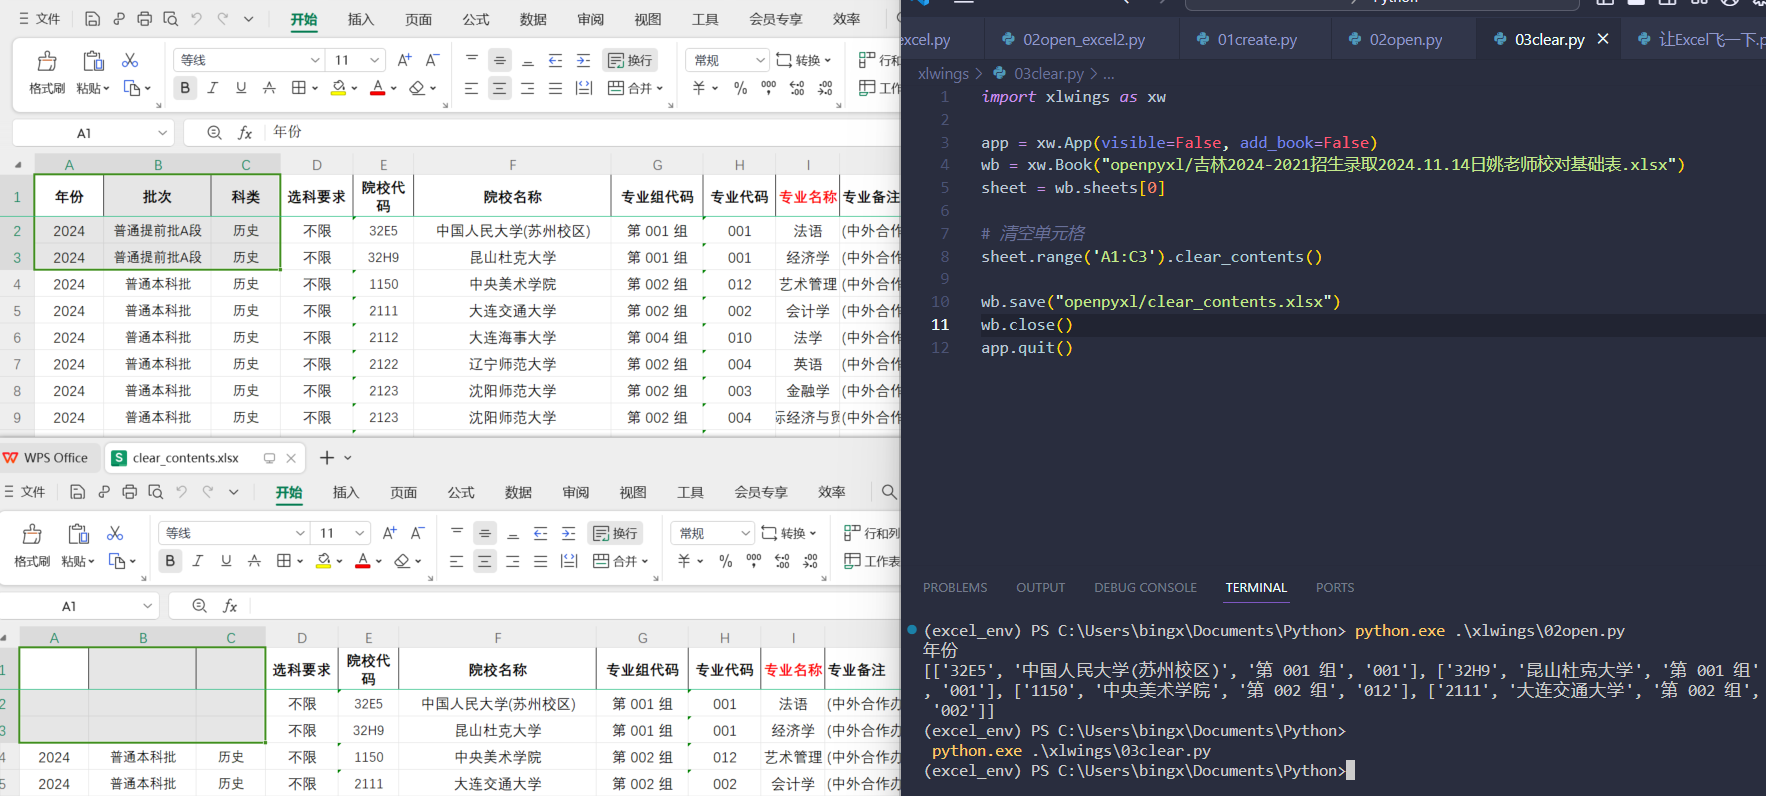
\includegraphics[width=0.6\textwidth]{part/自动化/办公自动化/pic/excel/xlwings/清空单元格演示.png}
    \caption{清空单元格演示}
    \label{fig:xlwings_清空单元格演示}
\end{figure}


\subsection{删除单元格}
删除单元格的方法是 \codeinline{range.delete(shift=None)},删除单元格后，影响到整个工作表的结构。
可选择向上或向左移动其余单元格。
\begin{enumerate}[label=\arabic*)]
    \item (\textcolor{red}{\textbf{不推荐}})\codeinline{shift=None}: 默认值，删除单元格后，不会移动其余单元格，
    但不一定有时候会移动其余单元格，不推荐使用

    \item \codeinline{shift='up'}: 删除单元格后，向上移动其余单元格
    \begin{figure}[htpb]
        \centering
        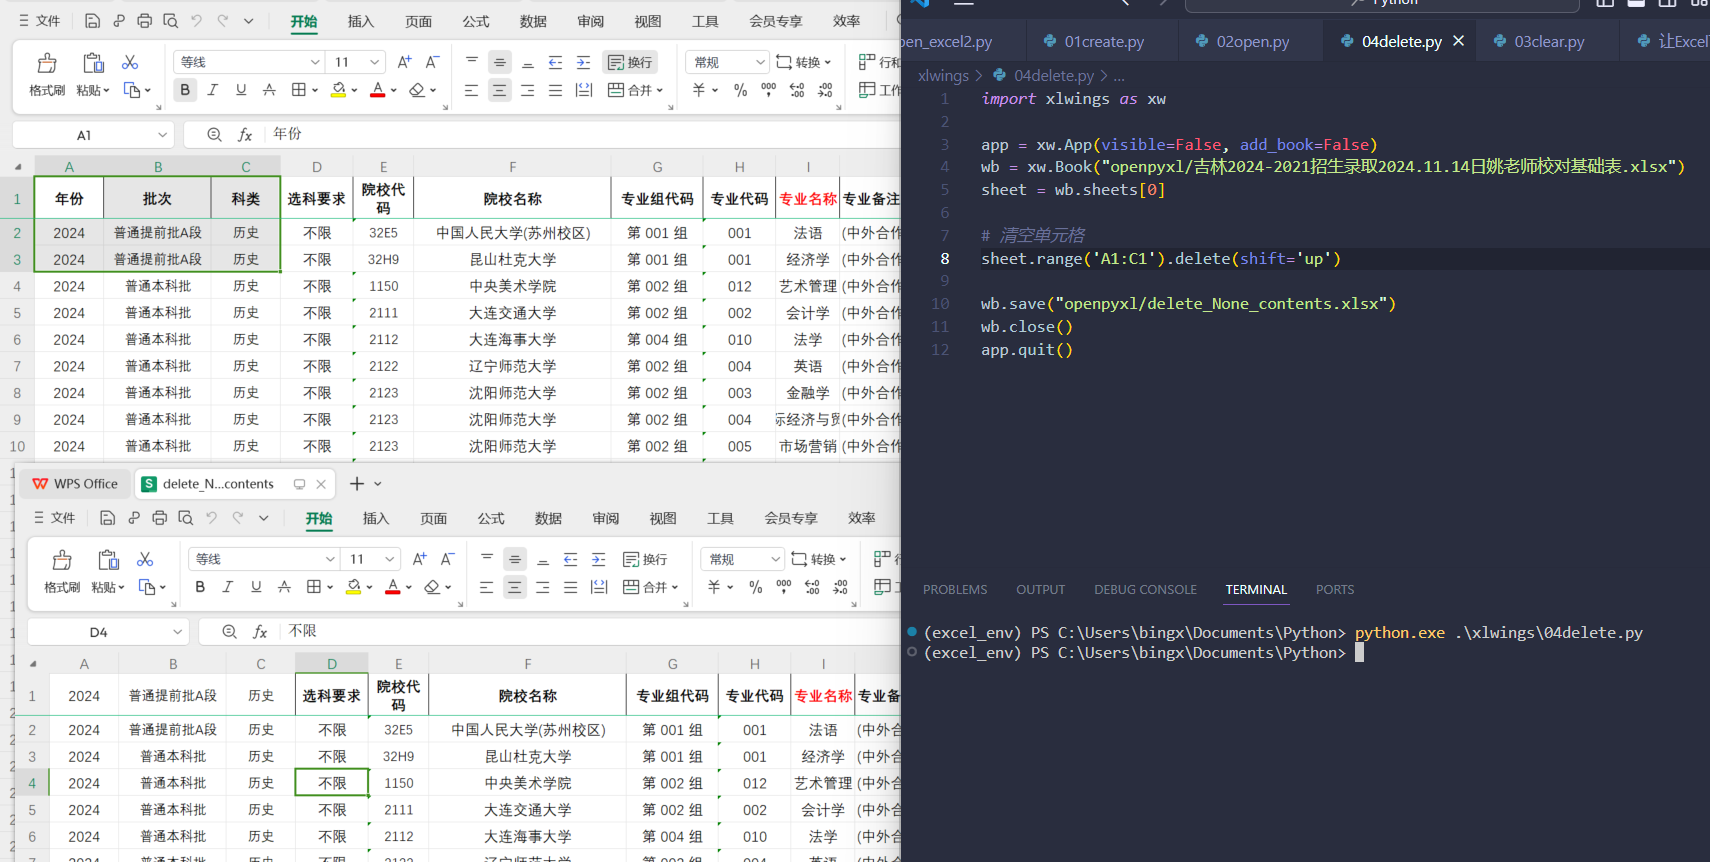
\includegraphics[width=0.6\textwidth]{part/自动化/办公自动化/pic/excel/xlwings/deleteshift=up效果.png}
        \caption{shift='up'效果}
        \label{fig:xlwings_deleteshift=up效果}
    \end{figure}
    
    \item \codeinline{shift='left'}: 删除单元格后，向左移动其余单元格
    \begin{figure}[htpb]
        \centering
        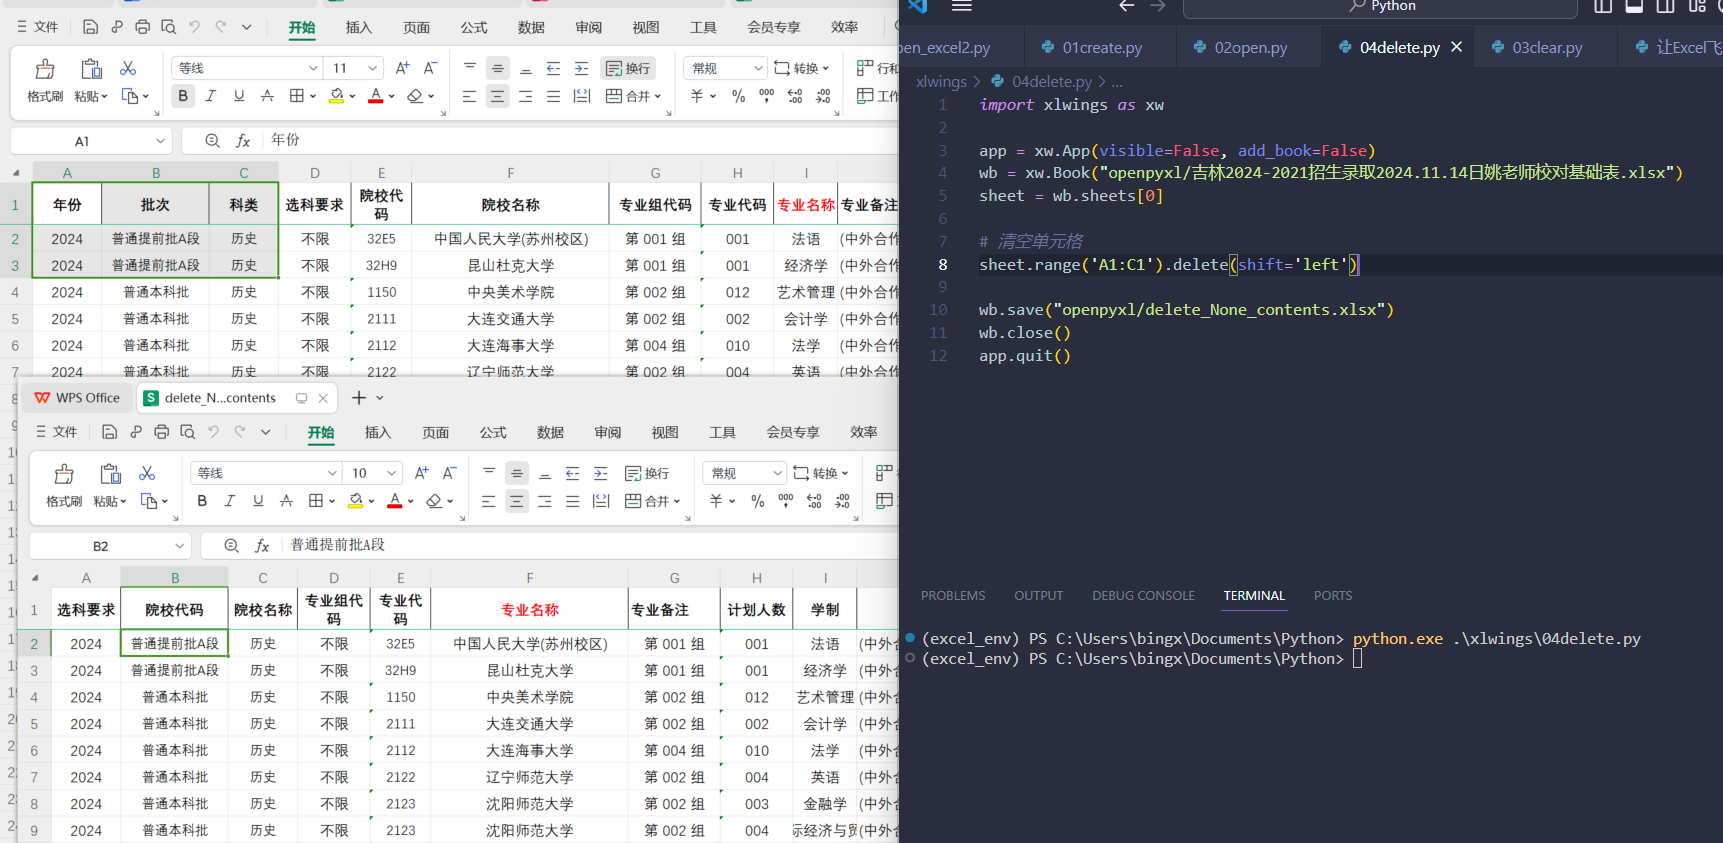
\includegraphics[width=0.6\textwidth]{part/自动化/办公自动化/pic/excel/xlwings/deleteshift=left效果.png}
        \caption{shift='left'效果}
        \label{fig:xlwings_deleteshift=left效果}
    \end{figure}
\end{enumerate}

\begin{lstlisting}[style=demostyle,numbers=none]
# 删除一行
sheet.range('1:1').delete()

# 删除一列
sheet.range('A:A').delete()
\end{lstlisting}


\subsection{插入单元格}
插入单元格的方法是 \codeinline{range.insert(shift=None)},插入单元格后，影响到整个工作表的结构。
可选择向下或向右移动其余单元格。
\begin{enumerate}[label=\arabic*)]
    \item (\textcolor{red}{\textbf{不推荐}})\codeinline{shift=None}: 默认值，插入单元格后，不会移动其余单元格，
    但不一定有时候会移动其余单元格，不推荐使用

    \item \codeinline{shift='down'}: 插入单元格后，向下移动其余单元格
    % \begin{figure}[htpb]
    %     \centering
    %     \includegraphics[width=0.6\textwidth]{part/自动化/办公自动化/pic/excel/xlwings/insertshift=down效果.png}
    %     \caption{shift='down'效果}
    %     \label{fig:xlwings_insertshift=down效果}
    % \end{figure}
    
    \item \codeinline{shift='right'}: 插入单元格后，向右移动其余单元格
    % \begin{figure}[htpb]
    %     \centering
    %     \includegraphics[width=0.6\textwidth]{part/自动化/办公自动化/pic/excel/xlwings/insertshift=right效果.png}
    %     \caption{shift='right'效果}
    %     \label{fig:xlwings_insertshift=right效果}
    % \end{figure}
\end{enumerate}

\begin{lstlisting}[style=demostyle,numbers=none]
# 插入一行
sheet.range('1:1').insert()

# 插入一列
sheet.range('A:A').insert()
\end{lstlisting}

\section{xlwings与panads的结合}
xlwings模块可以与pandas模块进行交互。

例如，用pandas模块创建数据表格，再用xlwings模块将表格写入工作簿，演示代码如下：
\begin{lstlisting}[style=demostyle,numbers=none]
import xlwings as xw
import pandas as pd
app = xw.App(visible=False)

# 创建一个新的工作簿
workbook = app.books.add()
worksheet = workbook.sheets.add('新工作表')

# 将DataFrame写入Excel
df = pd.DataFrame([[1, 2], [3, 4]], columns=['a', 'b'])
worksheet.range('B3').value = df # 在A1单元格写入DataFrame

# 保存工作簿
workbook.save(r'table.xlsx')
workbook.close()
app.quit()
\end{lstlisting}    
\begin{figure}[htpb]
    \centering
    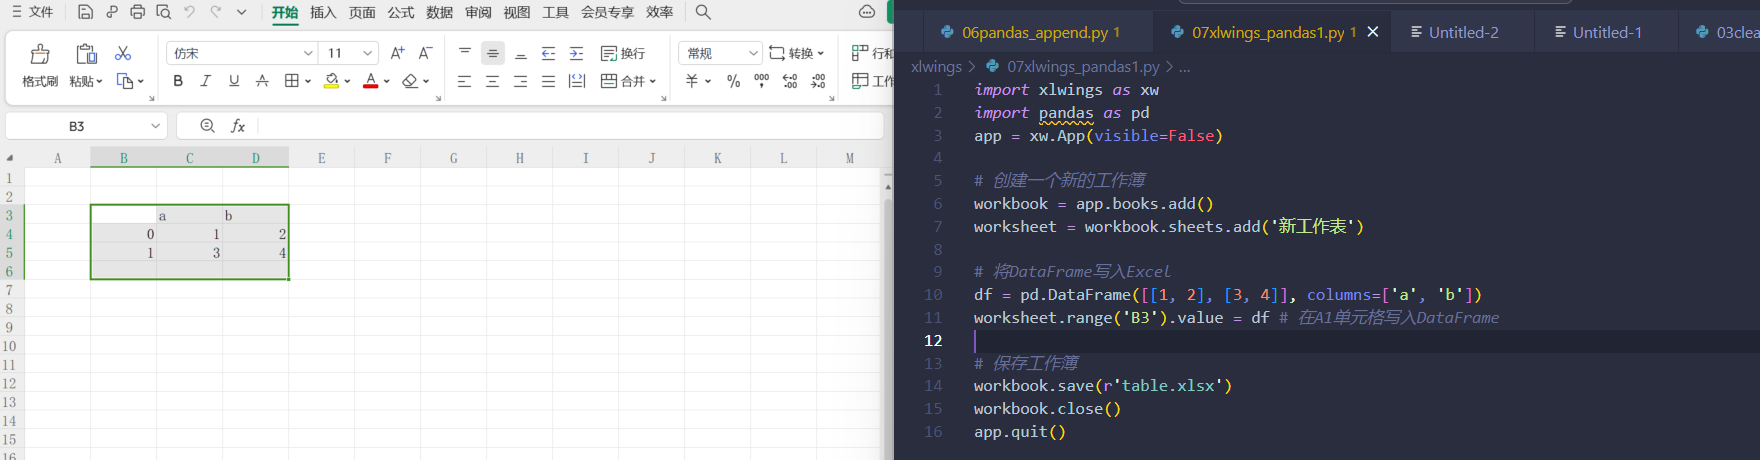
\includegraphics[width=0.6\textwidth]{part/自动化/办公自动化/pic/excel/xlwings/xlwings与pandas结合1.png}
    \caption{xlwings与pandas结合1}
    \label{fig:xlwings与pandas结合1}
\end{figure}
    


